% utk buat flowchart guna TikZ
\documentclass{standalone}

\usepackage{tikz}

\usetikzlibrary{shapes, arrows, positioning}

\begin{document}

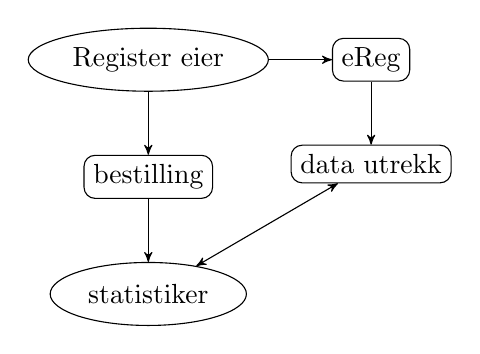
\begin{tikzpicture}
  [
  % block
  block/.style = {rectangle,
    rounded corners,
    draw, thin,
    node distance = 8mm,
    minimum height = 2mm},
  %bulat
  bulat/.style = {ellipse,
    draw, node distance = 8mm,
    minimum height = 8mm},
  % line
  line/.style = {draw, -stealth'},
  % distance
  node distance = 5mm,
  ]

  % nodes
  \node [block] (ereg) {eReg};
  \node [bulat, left= of ereg] (eier) {Register eier};
  \node [block, below= of ereg] (ut) {data utrekk};
  \node [block, below= of eier] (bestil) {bestilling};
  \node [bulat, below= of bestil] (stat) {statistiker};

  % Hvordan får man to noder på lik linje?

  % path
  \path [line] (eier) -- (ereg);
  \path [line] (ereg) -- (ut);
  \path [line] (eier) -- (bestil);
  \path [line] (bestil) -- (stat);
  \path [line, <->, >=stealth'] (ut) -- (stat);


\end{tikzpicture}

\end{document}